\documentclass[a4paper,10pt,twoside]{report}
\usepackage[T1]{fontenc}
\usepackage[frenchb]{babel} %active le mode français
\usepackage[latin1,utf8]{inputenc} % Mettre des accents
\usepackage[top=2cm , bottom=2cm , left=2cm , right=2cm]{geometry} %propriétés de notre page
\usepackage{amsmath} %liste de symboles et applications mathématiques
\usepackage{amsfonts} %idem
\usepackage{color} %Permet d'utiliser la couleur dans nos documents
\usepackage[usenames,dvipsnames]{xcolor}
\usepackage{listings} %Paquet de coloration syntaxique (langages)
\usepackage{hyperref} % Créer des liens et des signets 
\usepackage[babel=true]{csquotes} %permet les quotations (guillemets)
\usepackage{graphicx} %Importation d'image
\usepackage{fancyhdr} %en-tête et pieds de page+
\usepackage{lastpage} %permet d'obtenir le nombre total de page
\usepackage{multido}
%\usepackage{eurosym}
\usepackage{listingsutf8}
\usepackage{tikz}
\usepackage{ulem}
\usepackage{colortbl} %permet de mettre de personnaliser les colones des tabular
\usepackage{pdfpages}
\usepackage{appendix} %annexes
\setlength{\headheight}{15pt}
\lstset{language=C,
    breaklines=true,
	numbers=left,
	keywordstyle=\color{blue},
	commentstyle=\color{Gray},
	stringstyle=\color{red},
	tabsize=4,
	framexleftmargin=7mm,
	frame=single
	}
% Informations du rapport
\title {Rapport de TP \\ \textsc{Min-kernel VC}}
\author {Quentin Tonneau - Arthur Mahéo}
\date{}
\renewcommand{\thesection}{\arabic{section}}
%Propriétés des liens
\hypersetup{
colorlinks=true, %colorise les liens  
urlcolor= blue, %couleur des hyperliens 
linkcolor= blue,%couleur des liens internes
citecolor=black
} 
%\setlength{\parindent}{0cm}
\addto\captionsfrench{
	\renewcommand{\chaptername}{Partie}
}

\fancypagestyle{plain}
{

	\fancyhead{}
	\fancyfoot{}
	\fancyfoot[LO RE]{\textit{Q.Tonneau - A.Mahéo}}
	\lhead{X7IO010}
	\rhead{Université de Nantes}
	\chead{Algorithmes - Vertex Cover}
	\fancyfoot[LE]{\thepage}
	\fancyfoot[RO]{\thepage}
}
\begin{document}
\thispagestyle{empty}
\Large{\uline{
\noindent Arthur Mahéo}


\uline{Quentin Tonneau}}
\vfill
\begin{center}
\Huge{
 Rapport de Travaux Pratiques\\
 \textbf{Algorithmes de Résolution de Vertex Cover}}
 \vfill
 
\includegraphics[width=0.75\textwidth]{logo_univ_nantes.png}
 \vfill
\end{center}
X7IO040 \hfill Décembre 2012
%\newpage \pagestyle{empty}~
\tableofcontents
\newpage
\pagestyle{plain}
\chapter{Introduction}
  Nous essayons lors de ce projet d'implémenter plusieurs algorithmes de résolution du problème \textit{Min -Vertex Cover}, c'est à dire la couverture des arrêtes d'un graphe par un minimum sommets.
  L'exemple de la figure \ref{figure_exemple} nous montre un exemple de résultat. Le problème de Min-Vertex Cover est un des problèmes les plus difficiles connus $Min-Vertex-Cover \in NP-Conplet$.
  Pour obtenir le résultat le plus rapidement possible, nous essayons d'implémenter une heuristique simple, approximant la solution optimale avec un ratio de 2, puis à l'aide d'une recherche dichotomique sur le problème $PbD$ associé (\textit{Le graphe G peut-il être couvert par $k$ n\oe{}uds ?}), nous testons 
  d'une part un algorithme de kernelization (kernel-vc), et d'autre part un algorithme d'arbre de recherche borné (arb-vc).

    \begin{figure}[h]
    \centering
    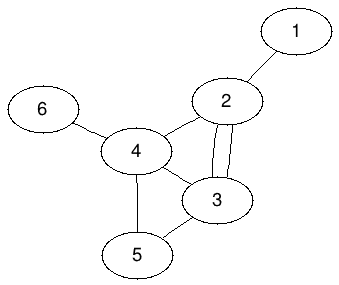
\includegraphics[width=0.45\textwidth]{grapheinitial}
    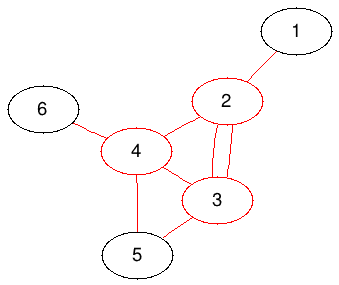
\includegraphics[width=0.45\textwidth]{graphefinal}\\
    \Huge{$Z=3$}
    \caption{Exemple d'instance - solution du problème \textit{Min - Vertex Cover}}
    \label{figure_exemple}
    \end{figure}

\chapter{Implémentations}
    \section{Génération de Graphe}
      La classe \textbf{Graph} représente un graphe à l'aide d'une liste d'adjacence. Une \texttt{map} possède en clé le numéro du n\oe{}ud, et en valeur associée la liste des n\oe{}uds liés.
      La suppression d'une arrête doit donc se faire dans les deux sens, ce qui est très rapide étant donné la structure associée. De même, la suppression d'un n\oe{}ud dans le graphe entraîne la suppression de toutes ses occurrences dans l'arbre.
      
        \subsection{Sommet de plus haut degré}
        Nous maintenons à jour le sommet de plus haut degré du graphe ainsi que sa valeur. Pour ce faire, et pour alléger la charge, à chaque fois que l'on enlève un n\oe{}ud ou une arête on passe un \textit{flag} à \textbf{vrai} et lors de l'appel de ce sommet, on le met à jour si nécessaire.
        
        \subsection{Couverture}
        Pour représenter notre couverture, nous diminuons notre graphe au fur et à mesure en lui enlevant des arêtes, voire des n\oe{}uds.
        
        Retirer une arêtes $(u.v)$ revient simplement à enlever l'occurrence de $u$ dans la liste d'adjacence de $v$ et vice-versa.
        
        Lorsque l'on retire un n\oe{}ud $u$, par contre, nous allons d'abord retirer ses occurernces dans l'ensemble de ses voisins du graphe avant de le supprimer.

    \section{Algorithme \textsc{2-Approx}}
    Cet algorithme permet d'approximer un \textsc{Min-VC} avec un ratio de 2. Il nous permettra donc de trouver des bornes à l'intervalle dans lequel lancer nos recherches pour les algorithmes de recherche arrivant par la suite.
    
    Son principe est :
    \begin{itemize}
        \item On prend une arête du graphe.
        \item On ajoute ses deux extrémités à la couverture.
        \item On répète jusqu'à couverture complète.
    \end{itemize}
    
    \section{Algorithme \textsc{ARB-VC}}
    Nous avons, dans ce cas, un algorithme exact, mais il requiert un paramètre $k$ du fait que c'est un problème de décision. \textsc{ARB-VC} résout : "existe-t-il une couverture de cardinalité $k$ pour G ?"
    Cet algorithme est basé sur le concept de l'arbre de recherche borné (ARB) et se comporte comme suit :
    \begin{itemize}
        \item On sélectionne le n\oe{}ud de plus haut degré $x$.
        \item On sélectionne l'ensemble de ses voisins $V$.
        \item On appelle \textsc{ARB-VC} sur, d'un côté $G' = G \textbackslash{} \{x\}$ avec un $k' = k - 1$ et, de l'autre, sur $G'' = G \textbackslash{} V$ avec $k'' = k - \#V$.
    \end{itemize}
    
    \section{Algorithme \textsc{Kernel-VC}}
    À nouveau un algorithme exact, qui répond à la même question que \textsc{ARB-VC}.
    \begin{itemize}
        \item On applique des règles de réduction à notre graphe :
        \begin{enumerate}
            \item Si un sommet est de degré 1, alors on ajoute son voisin à la couverture et réduisons $k$ de 1. Cela car le voisin en question est de degré au moins un.
            \item Si un sommet est de degré plus grand que $k$, on l'ajoute à la couverture --- car il n'existe pas de couverture de cardinalité $k$ sans lui.
        \end{enumerate}
        \item Une fois ces règles épuisée :
        \begin{itemize}
            \item si l'on a plus de $k^2$ arêtes dans notre graphe résiduel, on renvoie \textbf{faux} ;
            \item si $k = 0$ et que G n'est pas couvert, on renvoie \textbf{faux};
            \item si notre graphe est couvert on renvoie \textbf{vrai} ;
            \item sinon, on résout le noyau.
        \end{itemize}
    \end{itemize}
    Devant la lenteur d'une résolution du noyau avec un algorithme de type "brute force" nous avons décidé d'appeler \textsc{ARB-VC} à la rescousse.
    
    \section{Algorithme \textsc{Mon-Heuristique}}
    Notre heuristique est un approche naïve du problème et se comporte ainsi :
    \begin{itemize}
        \item Tant que l'on a pas couvert notre graphe, on ajoute son sommet de plus haut degré à notre couverture.
    \end{itemize}
    Sa complexité est en $O(n/2)$ puisque dans le pire cas, les sommets sont reliés 2 à 2, et il faut donc en retirer la moitié.  
    \section{Algorithme général}
    \paragraph{}L'algorithme principal est composé d'une boucle principale, permettant de générer tous les tableaux de $n=10$ à $n=1000$ selon l'incrémentation donnée dans le sujet.
  À chaque taille de graphe, une nouvelle boucle basée cette fois-ci sur les 5 probabilités données ($p=5/n$ à $p=0.2$), crée un graphe selon les conditions données, puis lance les deux algorithmes d'approximation (2-approx et Mon-heuristique). Une fois les bornes de la recherche dichotomique (\textbf{$res-2approx$} et \textbf{$\frac{res-2approx}{2}$} obtenues, nous recherchons la valeur optimale en lançant les deux fonctions de kernelization et d'arbre de recherche.
  
  \paragraph{}Pour arrêter les algorithmes après 3 minutes d'exécution, chaque fonction est lancée dans un thread différent, et un nouveau thread de chronométrage \textbf{tue} les deux fonctions si ces dernières sont toujours actives après la fin du temps impartit.
    
    \paragraph{} Si l'algorithme 2-Approx dépasse 3 minutes, alors nous sautons immédiatement à la probabilité / taille de graphe suivante. Si au cours de la recherche dichotomique l'algorithme kernel-vc ou arb-vc est tué, son exécution est alors interdite jusqu'à la prochaine dichotomie (et on essaye de terminer l'actuelle avec la fonction restante). 
    
    
\chapter{Résultats et Analyse}
    \section{Résultats}
    L'ensemble des tableaux de résultats se trouvent en annexe \ref{tableaux}. Nous avons choisi d’arrêter l'algorithme principal lorsque les fonction kernel-vc et arb-vc ne répondent plus dans une dichotomie.
    
    \section{Observations}
        On remarque lors de l'exécution de la boucle principale, que la réduction par kernel-vc avant l'exécution de l'arb-vc accélère grandement la vitesse de traitement de la dichotomie. Comme attendues, les valeurs de \textbf{kernel-vc} et \textbf{arb-vc} sont égales (lorsque les deux fonction aboutissent). La qualité de la fonction \textbf{2-approx} est perfectible, comme le montre notre (simple mais efficace) propre heuristique, qui de manière quasi systématique, trouve une borne supérieure de meilleur qualité dans un temps équivalent. En revanche, nous n'avons réussi à déterminer son ratio d'approximation, aussi la borne minimale actuelle reste $\frac{2-approx}{2}$   
\chapter{Conclusion}
Nous pourrions encore améliorer les temps de notre résolution, mais n'avons malheureusement pas eu le temps de terminer ces optimisations :
\begin{itemize}
    \item Implémenter une résolution polynomiale de tout graphe dont le degré maximum est deux. En effet, tant qu'il reste des sommets à traiter :
    \item Nous pourrions utiliser les résultats de \textsc{Mon heuristique} en tant que borne supérieur de l'intervalle de recherche pour $k$.
    \begin{enumerate}
        \item Soit nous avons une chaîne, et nous avons donc besoin de la moitié de ses sommets arrondie à l'inférieur pour la couvrir.
        \item Soit nous avons un cycle, et nous avons alors besoin de la moitié de ses sommets arrondie au supérieur pour le couvrir.
    \end{enumerate}
    \item Améliorer notre kernelisation en lui ajoutant des règles de réduction --- cf [1]:
    \begin{enumerate}
        \item Si on a un sommet de degré zéro, on le retire.
        \item On conserve la règle pour le degré un.
        \item Si on a un sommet de degré deux :
        \begin{itemize}
            \item si ses deux voisins sont adjacents : on ajoute les deux voisins à la couverture et passons à $k' = k - 2$.
            \item sinon, on \textit{contracte} ces sommets en un seul $v-u-w \rightarrow u'$, et travaillons sur $k' = k - 1$.
        \end{itemize}
        \item On conserve la règle pour les degrés supérieurs à $k$.
        \item Un fois ces règles épuisées :
        \begin{itemize} 
            \item si on a plus de $\frac{3k}{2} + k$ arêtes, on revoie \textbf{faux} ;
            \item si on a $k \leq 0$ et que le graphe n'est pas couvert, on revoie \textbf{faux} ;
            \item si le graphe est couvert on renvoie \textbf{vrai} ;
            \item sinon on résout le noyau.
        \end{itemize}
    \end{enumerate}
    \item \textit{Pour l'espace mémoire} Enlever par défaut les n\oe{}uds de degré zéro.
\end{itemize}
   
  \begin{appendices}
  \chapter{Tableaux de sortie des algorithmes}
    \label{tableaux}
    \begin{table}[h]
    \centering
    \begin{tabular}{||c||ccc||cccc||}
 \hline \hline 
 n=10&$m$&$\Delta (G)$&$d_M(G)$& Kernel-VC & ARB-VC & 2APPROX-VC & MonHeur-VC\\ \hline \hline
3/n&13&1.3&5&5&5&6&5\\
4/n&17&1.7&5&6&6&8&6\\
5/n&21&2.1&7&6&6&8&6\\
0.1&5&0.5&2&4&4&6&3\\
0.2&10&1&4&5&5&6&5\\
\hline \end{tabular}


    \caption{Résultats pour $n=10$}
    \end{table}
    
    
    \begin{table}[h]
    \centering
    \begin{tabular}{||c||ccc||cccc||}
 \hline \hline 
 n=20&$m$&$\Delta (G)$&$d_M(G)$& Kernel-VC & ARB-VC & 2APPROX-VC & MonHeur-VC\\ \hline \hline
3/n&26&1.3&5&9&9&14&10\\
4/n&37&1.85&6&11&11&16&12\\
5/n&44&2.2&7&12&12&18&12\\
0.1&18&0.9&3&9&9&16&8\\
0.2&37&1.85&6&11&11&16&12\\
\hline \end{tabular}


    \caption{Résultats pour $n=20$}
    \end{table}
   
   
   \begin{table}[h]
    \centering
    \begin{tabular}{||c||ccc||cccc||}
 \hline \hline 
 n=30&$m$&$\Delta (G)$&$d_M(G)$& Kernel-VC & ARB-VC & 2APPROX-VC & MonHeur-VC\\ \hline \hline
3/n&44&1.46667&6&15&15&26&17\\
4/n&55&1.83333&6&16&16&22&17\\
5/n&72&2.4&9&18&18&22&18\\
0.1&44&1.46667&6&15&15&26&17\\
0.2&87&2.9&9&19&19&26&19\\
\hline \end{tabular}


    \caption{Résultats pour $n=30$}
    \end{table}
    
    
    \begin{table}[h]
    \centering
    \begin{tabular}{||c||ccc||cccc||}
 \hline \hline 
 n=40&$m$&$\Delta (G)$&$d_M(G)$& Kernel-VC & ARB-VC & 2APPROX-VC & MonHeur-VC\\ \hline \hline
3/n&60&1.5&7&19&19&30&20\\
4/n&76&1.9&7&21&21&28&21\\
5/n&91&2.275&8&23&23&34&24\\
0.1&76&1.9&7&21&21&28&21\\
0.2&154&3.85&13&27&27&32&28\\
\hline \end{tabular}


    \caption{Résultats pour $n=40$}
    \end{table}
   
   
   \begin{table}[h]
    \centering
    \begin{tabular}{||c||ccc||cccc||}
 \hline \hline 
 n=50&$m$&$\Delta (G)$&$d_M(G)$& Kernel-VC & ARB-VC & 2APPROX-VC & MonHeur-VC\\ \hline \hline
3/n&78&1.56&8&24&24&38&26\\
4/n&107&2.14&8&28&28&44&30\\
5/n&131&2.62&9&30&30&42&32\\
0.1&131&2.62&9&30&30&42&32\\
0.2&239&4.78&15&35&35&44&37\\
\hline \end{tabular}


    \caption{Résultats pour $n=50$}
    \end{table}
    
    
    \begin{table}[h]
    \centering
    \begin{tabular}{||c||ccc||cccc||}
 \hline \hline 
 n=60&$m$&$\Delta (G)$&$d_M(G)$& Kernel-VC & ARB-VC & 2APPROX-VC & MonHeur-VC\\ \hline \hline
3/n&86&1.43333&7&28&28&44&29\\
4/n&116&1.93333&10&32&32&44&33\\
5/n&156&2.6&12&36&36&46&38\\
0.1&181&3.01667&11&38&38&48&41\\
0.2&338&5.63333&17&44&44&56&46\\
\hline \end{tabular}


    \caption{Résultats pour $n=60$}
    \end{table}
    
    \begin{table}[h]
    \centering
    \begin{tabular}{||c||ccc||cccc||}
 \hline \hline 
 n=70&$m$&$\Delta (G)$&$d_M(G)$& Kernel-VC & ARB-VC & 2APPROX-VC & MonHeur-VC\\ \hline \hline
3/n&97&1.38571&7&33&33&52&34\\
4/n&139&1.98571&8&38&38&56&40\\
5/n&160&2.28571&9&38&38&54&39\\
0.1&217&3.1&12&43&43&60&44\\
0.2&503&7.18571&24&52&52&64&54\\
\hline \end{tabular}


    \caption{Résultats pour $n=70$}
    \end{table}
    
    \begin{table}[h]
    \centering
    \begin{tabular}{||c||ccc||cccc||}
 \hline \hline 
 n=80&$m$&$\Delta (G)$&$d_M(G)$& Kernel-VC & ARB-VC & 2APPROX-VC & MonHeur-VC\\ \hline \hline
3/n&104&1.3&6&37&37&54&40\\
4/n&153&1.9125&9&39&39&62&42\\
5/n&178&2.225&11&45&45&64&47\\
0.1&303&3.7875&16&52&52&70&52\\
0.2&638&7.975&24&62&62&76&64\\
\hline \end{tabular}


    \caption{Résultats pour $n=80$}
    \end{table}
    
    \begin{table}[h]
    \centering
    \begin{tabular}{||c||ccc||cccc||}
 \hline \hline 
 n=90&$m$&$\Delta (G)$&$d_M(G)$& Kernel-VC & ARB-VC & 2APPROX-VC & MonHeur-VC\\ \hline \hline
3/n&138&1.53333&8&43&43&64&44\\
4/n&176&1.95556&10&47&47&68&49\\
5/n&208&2.31111&10&49&49&70&51\\
0.1&402&4.46667&15&61&61&78&63\\
0.2&806&8.95556&29&71&71&86&74\\
\hline \end{tabular}


    \caption{Résultats pour $n=90$}
    \end{table}
    
    \begin{table}[h]
    \centering
    \begin{tabular}{||c||ccc||cccc||}
 \hline \hline 
 n=100&$m$&$\Delta (G)$&$d_M(G)$& Kernel-VC & ARB-VC & 2APPROX-VC & MonHeur-VC\\ \hline \hline
3/n&129&1.29&7&45& nrp&72&48\\
4/n&201&2.01&9&53& nrp&80&55\\
5/n&275&2.75&11& nrp& nrp&84&63\\
0.1&527&5.27&19&70&70&90&74\\
0.2&1050&10.5&33&82&82&94&86\\
\hline \end{tabular}


    \caption{Résultats pour $n=100$}
    \end{table}
    
    \begin{table}[h]
    \centering
    \begin{tabular}{||c||ccc||cccc||}
 \hline \hline 
 n=120&$m$&$\Delta (G)$&$d_M(G)$& Kernel-VC & ARB-VC & 2APPROX-VC & MonHeur-VC\\ \hline \hline
3/n&184&1.53333&8&56& nrp&82&56\\
4/n&267&2.225&11& nrp& nrp&96&66\\
5/n&300&2.5&11& nrp& nrp&98&72\\
0.1&664&5.53333&22& nrp& nrp&106&88\\
0.2&1419&11.825&38&98&98&112&101\\
\hline \end{tabular}


    \caption{Résultats pour $n=120$}
    \end{table}
    \end{appendices}
\end{document}



